\documentclass{article}

\usepackage{graphics}
\usepackage{amsmath}
\usepackage{amsthm}
\usepackage{amsfonts}

\title{The Cutoff Phenomenon of Passive Scalars Advected by Chaotic Maps with Small Diffusion }
\author{Tzu-Chen Liang}
\date{\today}

% End of Preamble

\newtheorem{example}{Example}
\newtheorem{assumption}{Assumption}
\newtheorem{definition}{Definition}
\newtheorem{theorem}{Theorem}

\begin{document}

\maketitle

\begin{abstract}

We numerically study the decay of the variance of a passive scalar function in a chaotic flow when the diffusibility tends to zero and link the result to the well-known cutoff phenomenon found in Markov chain simulations. An efficient and parallelizable Markov chain model is built to simulate the chaotic map with small diffusion. The sequence of Markov chains generated by reducing the numerical diffusion or improving the resolution presents a cutoff when the underlying map is chaotic. This result points out one possibility of the source of cutoff phenomenon. 



\end{abstract}

%%%%%%%%%%%%%%%%%%%%%%
\section{Introduction}
\label{Introduction}
%%%%%%%%%%%%%%%%%%%%%%
The problem of how chaotic advection mixes a passive scalar function has attracted more research efforts in recent years\cite{Ottino2004}. The main issues in this field are: how to measure the thoroughness of the mixing, how the mixing process changes qualitatively and quantitatively when the diffusibility tends to zero, and how to enhance the overall mixing process by designing the map which produces chaotic advection. Unfortunately, we have only fractional understanding on most of these topics. In spite of the fact that the detail mechanism of mixing is unclear, the non-trivial mixing process has been observed in experiments \cite{Rothstein1999}\cite{Voth2002} and can be simulated by large-scale computations \cite{Tsang2005}. In this paper we build a linear Markov chain model to simulate the chaotic mixing with small diffusion. This simple and parallelizable linear model not only  captures the multi-stage feature of a chaotic mixing process, but also generates a series of finite Markov chains which presents a cutoff. Cutoff is a well-known phenomenon widely observed in Markov chain simulations\cite{Diaconis1996}\cite{Diaconis2005}\cite{Diaconis1986}\cite{Diaconis1990}. Researches are focused on how it happens by examining the special eigen structure of the underlying Markov matrices, but the physical explanation of what causes the cutoff is void. We build the connection between the cutoff phenomenon and the mixing process on the zero diffusivity limit, and suggest one possible reason that causes a cutoff.



\paragraph{The Multi-stage Feature of Chaotic Mixing Processes}
A widely observed phenomenon in the chaotic mixing process when small diffusibility exists is the two or three-stage transition\cite{Thiffeault2003-13}\cite{Fereday2002}\cite{Antonsen1996}. The map does not mix the scalar function with 
a constant rate in general. When the variance of the scalar function is measured during the mixing process, one can in general observe a relatively flat decay followed by a super-exponential change, and then finally it tends to a exponential decay. People are interested in when these transitions happen, why they happen, and how to predict the slope of the 
exponential region. A good review and physical interpretation can be found in \cite{Thiffeault2004}.  

\cite{Thiffeault2003-13} studies these properties for a modified Arnold's cat map. Analytical formulas are given to predict the transitions as well as the slopes. However, it is because the linear part of this map stretches very fast (with an eigenvalue 2.618) and the chaotic part is relatively small so that the three phases are separated clearly. The same results cannot be applied to, for example, standard map, although the only difference between the standard map and the modified Arnold's cat map is in the linear part.

As for the exponential decay part, people are still debating about whether the decay rate goes to zeros in the zero diffusivity limit or it tends to a constant independent of the diffusibility \cite{Thiffeault2004}\cite{Tsang2005}. Theoretical analysis shows both of them are possible for different chaotic flows \cite{Haynes2005}.  
 
The difficulty of the numerical studies of the above problems is the small diffusibility usually means fine grids in solving the advection-diffusion equation or simulating the map. Some of the simulation results which conclude the proportional relation 
between the stationary decay rate and the diffusibility are actually because of lacking in resolution \cite{Cerbelli2003}\cite{Pikovsky2003}. \cite{Tsang2005} uses a simple and parallelizable numerical strategy which can run up to $6 \times 10^4$ by $6 \times 10^4$ grids to show the decay rate of a certain chaotic map tends to a constant. However, there are also converse evidence found in other maps. 

In this paper, we focus on the mixing process of standard map with small diffusivity. We build a similar numerical strategy to simulate the map with very high resolution (up to $8 \times 10^4$ by $8 \times 10^4$ grids). We run simulations in different resolutions with different numerical and physical diffusions to demonstrate the accuracy of this model, and we numerically shows that the sequence of Markov chains presents a cutoff, which qualitively characterizes the mixing process when the diffusion tends to zero. 




\paragraph{Cutoff Phenomenon in Markov Chain Simulations}
A somewhat more surprising fact is this two or three-stage transition, especially the super-exponential decay phase also occurs in some simple linear systems, and they have been observed and named cutoff phenomenon in Markov chain simulations. This phenomenon is firstly found by Diaconis and Shahshahani in \cite{Diaconis1981}. Later some more examples are given by Aldous and Diaconis in \cite{Diaconis1986}. The well-known examples are the birth-death chain \cite{Diaconis2005} and the
riffle shuffle problem\cite{Diaconis1996}\cite{Diaconis2001}. For a birth-death chain problem, one can creates a cutoff simply by a Markov chain system with only several states. As for the riffle shuffle problem, the number of states need to go up to extremely large ($n!$ when there are $n$ cards). 


Whether the cutoff phenomenon happens also depends on the measure one uses\cite{Diaconis2005}. It is quite possible that 
a sequence of Markov chains presents a cutoff if the total variational distance is used, while it decays smoothly in the separation measure, or the other way around. Exactly the same thing occurs in the chaotic mixing process with small diffusion. For example, if one uses the mix-variance suggested in \cite{Mezic2005} to measure the mixing of standard map (with or without diffusion), it shows no super-exponential region, which is very different from the trajectory
if one measures the variance of the scalars. 

These coincidences makes us to think of the connection between them. The idea to build this connection is that we think any chaotic map can be represented as a infinity dimensional linear system by obtaining the Frobenius-Perron operator. And then we find the finite dimensional approximation of this operator to construct a finite dimensional Markov chain. This Markov chain system is obviously an approximation of the chaotic map. By adjusting the number of grids we use in descretlizing the phase space, a sequence of Markov chain models with ascending accuracy can be built. Physically this is like to decrease the numerical diffusibility caused by the descretlization. We then show this sequence of Markov chains presents a cutoff. The importance of this result is it suggests a cutoff can be formed by the sequence of Markov chain models with accending accuracy, or equivalently, decending numerical diffusibility, to a chaotic map. 

This paper is organized as the follows: Section \ref{Notations} we introduce the notations, and since the cutoff phenomenon of both chaotic mixing process and Markov chain system are highly related to the measure, section \ref{Measure for Scalar Functions} is to describe the various measures for both cases. Section \ref{The Markov Chain Model of a Map} explains how we build the Markov chain system for a given chaotic map, and section \ref{The Cut-off Phenomenon of Chaotic Mixing Processes} we use simulations to show the sequence of Markov chain models actually present a cutoff phenomenon. Then a conclusion is given in \ref{Conclusions}. 
 
%\paragraph{Measure of Mixing}
%There is no consensus on how to measure the mixing of a passive
%scalar function so far\cite{Mezic2005}. \cite{Wiggins2004} builds
%the hierarchical structure of maps with different mixing properties
%qualitatively and characterizes that the most desired mixer has the
%property called Bernoulli, but it does not tell anything about how
%fast it mixes. Maximum entropy approach has been used in, for
%example \cite{DAlessandro1999}, as a measure of mixing. However,
%this measure is a property of the dynamical system and independent
%of the initial configuration of the scalar function, thus it is not
%so useful when one wants to design a mixing protocol for a
%particular initial scalar function, and which is quite common in
%practice. The simplest and widely used way is to measure the $L^2$
%norm or the variance of the scalar function \cite{Ashwin2002},
%\cite{Thiffeault2003-13},\cite{Thiffeault2003-309}, []. This
%approach can be applied when the mixing process is diffusive or
%artificial diffusion is added, otherwise the function is never mixed
%in the sense of this measure. This is in general not a problem in
%practice because the true system is always diffusive. Nonetheless,
%we still want to somehow distinguish the difference between a smooth
%scalar function and a highly oscillated one. Clearly $L^2$ norm and
%the variance measures are not helpful here. \cite{Mezic2005} defines
%a new mix-norm, which resolves this problem and can be served as a
%measure of mixing for both diffusive and non-diffusive systems. As
%the author stated, this norm is equivalent to the Sobolev norm with
%index $s = -\frac{1}{2}$, i.e. it is diagonal in the frequency
%domain and weights less on the high wave number terms. So even when
%a volume-preserved map is applied to the scalar function, one can
%still observe the change of this mix-norm. In fact, any Sobolev norm
%with negative $s$ index have this desired property. Hence there are
%not much difference in choosing the mix-norm or any of these Sobolev
%norm when measuring mixing. In this paper, we will compare these
%mixing measures and suggest a more natural one, called
%diffusion-norm. Physically, it measures the $L^2$ norm when one
%diffuses the scalar function for time duration $t$ and diffusive
%rate $D$. The advantage of this measure is for a real system, these
%physical parameters actually exist and the mixing in the
%corresponding length-scale is the one we care. This diffuse-norm is
%also diagonal in frequency domain and decreasing when the wave
%number gets higher, so it preserves the property of the mix-norm and
%also gives the freedom of adding the important physical quantities
%one want to measure.







%%%%%%%%%%%%%%%%%%%
\section{Notations}
\label{Notations}
%%%%%%%%%%%%%%%%%%%
\subsection{Frobenious-Perron Operator}
Let $T^2 =[0,1]\times[0,1]$ be a 2-dimensional torus. We consider $c:T^2 \rightarrow \mathbb{R}$ to be the density field or the scalar function. $S:T^2\rightarrow T^2$ is a non-singular (invertible measure-preserving) transformation, or a map. Then the Frobenious-Perron operator $[P]:L_{T^2}^2\rightarrow L_{T^2}^2$ is defined as
\begin{eqnarray}
\label{FPoperator}
  [P]c(\mathbf{x})=c(S^{-1}(\mathbf{x}))
\end{eqnarray}
where $\mathbf{x}=(x,y)$. A continuous-time map $S_c: T^2 \times \mathbb{R} \rightarrow T^2$ is the coordinate transformation $S_c: \mathbf{x}_0 \mapsto S_c(\mathbf{x}_0,t) $ for some $\mathbf{x}_0$ and time $t$. Similarly, the continuous-time Frobenious-Perron operator is written as $[P(t)]:L_{T^2}^2\rightarrow L_{T^2}^2$, which satisfies $[P(t)]c(\mathbf{x}) = c(S_c(\mathbf{x},-t))$.

$[M(D,t)]: L_{T^2}^2  \rightarrow L_{T^2}^2$ is the diffusion operator, where $D$ and $t$ are the diffusibility rate and time. We define $c'(\mathbf{x}) = [M(D,s)]c(\mathbf{x})$, where $c'(\mathbf{x})= u(\mathbf{x},s)$ and $u:L_{T^2}^2 \times \mathbb{R} \rightarrow \mathbb{R} $ is the solution of the following partial differential equation,
   \begin{eqnarray}
   \label{diffusion equation}
    u_{t} = D(u_{xx}+u_{yy})        \\
    u(x,y,0) = c(x,y)      \nonumber\\
    u(1,y,t) = u(0,y,t)    \nonumber\\
    u(x,1,t) = u(x,0,t)    \nonumber
   \end{eqnarray}
In order to simulate both advection and diffusion, we need to solve the diffusion equation (\ref{diffusion equation}) under a given map. For a continuous-time map $S_c$, define $v(S_c(\mathbf{x},t),t) = \frac{d}{dt}S_c(\mathbf{x},t)$ to be the vector field of it. Then $[P(D,t)]:L_{T^2}^2\rightarrow L_{T^2}^2$ is the advection-diffusion operator. $c'(\mathbf{x}) = [P(D,s)]c(\mathbf{x})$, where $c'(\mathbf{x})= u(\mathbf{x},s)$ is the solution of the following PDE at time $s$,
   \begin{eqnarray}
   \label{advection-diffusion equation}
    u_{t} + v \cdot \nabla{u}  = D(u_{xx}+u_{yy})        \\
    u(x,y,0) = c(x,y)      \nonumber\\
    u(1,y,t) = u(0,y,t)    \nonumber\\
    u(x,1,t) = u(x,0,t)    \nonumber
   \end{eqnarray}
Equation (\ref{advection-diffusion equation}) is called advection-diffusion equation. In discrete-time case, for the time interval $\Delta t$ it is simply $[P(D,\Delta t)]:L_{T^2}^2\rightarrow L_{T^2}^2$ and
\begin{eqnarray}
\label{PDdef}
 [P(D,\Delta t)]c(\mathbf{x})= [M(k,\Delta t)]c(S^{-1}(\mathbf{x}))
\end{eqnarray}
In this paper, we do not solve (\ref{advection-diffusion equation}) directly even if the given map is continuous. Instead, we use the following approximation,
\begin{eqnarray}
[P(D,\Delta t)]c(\mathbf{x}) &\approx& [M(k,\Delta t)]c(S_c^{-1}(\mathbf{x}, -\Delta t))\\
                             & =     & [M(k,\Delta t)][P(\Delta t)]c(\mathbf{x})
\end{eqnarray}
i.e. the advection and diffusion steps are separated. This approach has been used in, for example, \cite{Tsang2005}\cite{Thiffeault2003-13}.(Need some more reference)  





$P_h: \mathbb{R}^{1/h^2} \rightarrow \mathbb{R}^{1/h^2} $ and $M_h: \mathbb{R}^{1/h^2} \rightarrow \mathbb{R}^{1/h^2}$ are the finite dimensional approximations of Frobenious-Perron and diffusion operators on regular meshes with size $h$. The same as the operator $[M(D,t)]$, we use $M_h(D,t)$ to represent the diffusion operator with diffusion rate $D$ and diffuse time $t$.


\subsection{Finite Markov Chains}
Let $\chi$ be a finite space of cardinality $|\chi|=n$. A discrete time Markov chain is a sequence of $\chi$-valued random variables $(W_l)_0^{\infty}$ satisfying
\begin{eqnarray*}
 &\mathbf{Prob}(W_l = w_l | W_{l-1} = w_{l-1},W_{l-2} = w_{l-2},...,W_0 = w_0)  \\
 &=\mathbf{Prob}(W_{l} = w_l | W_{l-1} = w_{l-1})
\end{eqnarray*}
for all $w_i \in \chi$ with $0 \le i \le l$ and $l\ge 0$. A Markov chain is time homogeneous if the quantity in the right hand side above is independent of $l$. In this case, such a Markov chain is specified by the initial distribution (the distribution of $W_0$) and the one-step transition kernal or Markov kernal $K\,:\, \chi \times \chi \rightarrow [0,1]$, which is defined by
\begin{eqnarray*}
\forall x,y \in \chi, \,\,\, K(x,y)=\mathbf{Prob}(W_{l+1} = y |
W_{l} = x)
\end{eqnarray*}
For any Markov chain $(W_l)_0^{\infty}$ with transition matrix $K$ and initial distribution $w^0$,  $\mathbf{Prob}(W_0=x)=w^0(x)$ for all $x \in \chi$, the distribution of $W_l$ is given by
\begin{eqnarray}
\label{Kevolvedistribution} \forall x\in \chi \,\,\, w^l(x) =
\mathbf{Prob}\{W_l=x\}=(w^0 K^l)(x)=\sum_{y\in \chi} w^0(y)K^l(y,x)
\end{eqnarray}
where $K^l$ is a matrix defined iteratively by
\begin{eqnarray*}
\forall x,y \in \chi \,\,\, K^l(x,y)=\sum_{z \in
\chi}K^{l-1}(x,z)K(z,y)
\end{eqnarray*}


A Markov kernal $K$ on $\chi$ is said to be irreducible if for any $x,y$ there exists $j = j(x,y)$ such that $K^j(x,y)>0$. A state $x\in\chi$ is called aperiodic if $K^l(x,x)>0$ for sufficiently large $l$, and $K$ is called aperiodic if all states are aperiodic. Under the assumption of irreducibility of $K$, there exists a unique
stationary distribution $\pi$ satisfying $\pi K =\pi$

If $K$ is irreducible and aperiodic, then
\begin{eqnarray*}
\forall x,y \in \chi \,\,\, \lim_{l \rightarrow \infty}
K^l(x,y)=\pi(y)
\end{eqnarray*}

We work on the ($n$-dimensional) Hilbert space $\ell^2(\pi)$. The adjoint operator of $K$ is $K^*$,
\begin{eqnarray*}
\label{Kadjoint}
  K^*(x,y) = \pi(y)K(y,x)/\pi(x)
\end{eqnarray*}
$K^*$ is also a Markov operator. The Markov process associated with $K^*$ is the time reversal of the process associated with $K$. If a measure $\mu$ has density $f$ with respect to $\pi$, that is, if $\mu(x)=f(x)\pi(x)$, then $\mu K$ has density $K^*f$ with respect to $\pi$. Thus acting by $K$ on a measure is equivalent to acting by
$K^*$ on its density with respect to $\pi$.

The above observation says to evolve the density $f$ forward in time, $K^*$ is the operator one needs, i.e.,
\begin{eqnarray}
\label{fevolve}
f^l(x) =  (K^*f^{l-1})(x)= \sum_{y \in \chi}
K^*(x,y)f^{l-1}(y)
\end{eqnarray}
where $f^l$ and $f^{l-1}$ are the densities of $w^l$ and $w^{l-1}$
with respect to $\pi$. The probabilistic interpretation of a Markov matrix is almost never used in this paper. We apply (\ref{fevolve}) to scalar functions and read $K^*$ as a linear opetator.    

\subsection{The Norms for Probability Measures}

Let $\Omega$ be a finite set, and $\pi$ a no where vanishing finite measure on $\Omega$. For $1 \le p \le \infty$ and any (complex-valued) function $f$ on $\Omega$, the $\ell^p(\pi)-norm$ (or briefly the $\ell^p-norm$, if there is no confusion) of $f$ is defined by
\begin{eqnarray}
\label{lpnorm}
  \|f\|_p = \|f\|_{\ell^p(\pi)} =   \left\{ \begin{array}{cc}
                 \left(   \sum_{x \in \Omega} |f(x)|^p \pi(x) \right)^{1/p} &\mbox{, if } 1\le p<\infty\\
                 \max_{x \in \Omega} &\mbox{, if } p = \infty\\
              \end{array} \right.
\end{eqnarray}

We can use the definition of $\ell^p(\pi)-norm$ to measure a scalar function on $L^{2}_{T^2}$ by simply replace the summation by an integral over $T^2$. To do that numerically, however, we use regular square mesh grids with size $h$ by $h$ on $T^2$, and define a function $[d_h]: T^2 \rightarrow \mathbb{R}^{1/h^2}$ as
\begin{eqnarray}
[d_h]c(\mathbf{x}) = c
\end{eqnarray}
where $c_i = \int_{a_i} c(\mathbf{x}) \text{d}a$ for $i = 1,2,...1/h^2$, and $a_i$ stands for the $i_{th}$ grid. So $c$ is the finite dimensional approximation of $c(\mathbf{x})$ on the regular grids with size $h$, and then (\ref{lpnorm}) is applied by setting $f(x) = c_x, \forall x \in \Omega $ and suitable $\pi$.


Let $\mu$, $\nu$ and $\pi$ be finite measure on $\Omega$ and assume that $\pi$ is positive everywhere. The $\ell^p(\pi)-distance$ (or briefly the $\ell^p-distance$) between $\mu$ and $\nu$ is defined to be 
\begin{eqnarray}
 d_{\pi,p}(\mu,\nu) = \| f-g \|_{\ell^p(\pi)} 
\end{eqnarray}
where $f$ and $g$ are corresponding densities of $\mu$ and $\nu$ with respect to $\pi$, which means $\mu = f\pi$ and $\nu = g\pi$. According to the definitions, if $\mu(\Omega) = \nu(\Omega)$, then

\begin{eqnarray}
 d_{\pi,1}(\mu,\nu)=\sum_{x \in \Omega}|\mu(x)-\nu(x)| \equiv  2  d_{TV}(\mu,\nu)
\end{eqnarray}  
where $d_{TV}$ is the total variance distance. Similarly, 

\begin{eqnarray}
\label{L2distance}
 d_{\pi,2}(\mu,\nu) = \left(  \sum_{x \in \Omega} \left| \frac{\mu(x)}{\pi(x)}-\frac{\nu(x)}{\pi(x)} \right|^2 \pi(x) \right)^{1/2}
\end{eqnarray}




\subsection{Cutoff Phenomenon}
We also state the definition of a cutoff given by Diaconis in
\cite{Diaconis2005}. Assume that, to any finite set $\Omega$ and any
pair of probability measures $\mu$, $\nu$ on $\Omega$ is associated
a real number $D(\mu,\nu)$ such that $D(\mu,\nu)\in [0,1]$,

\begin{eqnarray}
\max_{\Omega,\mu,\nu} D(\mu,\nu) = 1
\end{eqnarray}
and $D(\mu,\nu)=0$ if and only if $\mu=\nu$. Consider a sequence of
(finite) probability spaces $(\Omega_n,\nu_n)$, $n=1,2,...$, each
equipped with a sequence of probability measure $\mu^k_n$,
$l=0,1,...$, such that
\begin{eqnarray}
\lim_{k \rightarrow \infty} D(\mu^k_n,\nu_n)=0
\end{eqnarray}
The definition of a cut-off is,

\begin{definition}
\label{cutoffdefition}
(Diaconis) A family $(\Omega_n,\nu_n, (\mu^k_n)_{k=0,1,...})_{n=1,2,...}$
presents a D-cut-off if there exists a sequence $(t_n)$ of positive
reals such that, for any $\epsilon \in(0,1)$,
\begin{enumerate}
  \item $\lim_{k \rightarrow \infty}D(\mu^{k_n}_n,\nu_n) = 0 \mbox{ if }
  k_n>(1+\epsilon)t_n$
  \item $\lim_{k \rightarrow \infty}D(\mu^{k_n}_n,\nu_n) = 1 \mbox{ if }
  k_n<(1-\epsilon)t_n $
\end{enumerate}
\end{definition}

One example of a family of $\varphi^k_n \equiv D(\mu_k^n,\nu_n)$ sequence
is shown in figure \ref{democutoff1} (a). Define the D-mixing time
\begin{eqnarray}
\label{Dmixingtime}
\tau^D_n=\tau^D_n(\epsilon) = \inf\{k\,:\,D(\mu_k^n,\nu_n) \le \epsilon\}
\end{eqnarray}
If we normalize the trajectories in figure \ref{democutoff1} (a) by their $\tau_n^D(0.5)$, the
normalized trajectories are shown in figure \ref{democutoff1} (b).


Definition \ref{cutoffdefition} restricts the maximum of diatance $D$ to be $1$.
However, this can be easily extended to the case where $D$ is unbounded \cite{Diaconis2005},
In this paper, we are mainly interested in the following two cases
\begin{eqnarray}
\label{normweuse}
 D(\mu,\nu) = d_{\nu,1}(\mu,\nu)\\ 
 D(\mu,\nu) = d_{\nu,2}(\mu,\nu)\nonumber
\end{eqnarray}
In the second case, the limit value $1$ in definition \ref{cutoffdefition} should be replaced by $\infty$.
An example of this kind of cutoff trajectories and the normalized one are shown in figure \ref{democutoff2} (a)(b). \cite{Chen2006} discusses the
$L^2$ cut-off phenomenon in detail. Discussions about other distances can be found in \cite{Diaconis2005}\cite{Chen2006}\cite{LSaloff-Costt1997}, etc.


One shall remember that although the distances in (\ref{normweuse}) are defined for two probability measures, we actually more interested in the scalar density functions defined by $f =\mu / \nu $. When this is applied and $h \rightarrow 0$ on regular grids, the two distances in (\ref{normweuse}) are the same as the $L^1$ and $L^2$ norms of a continuous function (with some scaling).  



\begin{figure}
 \centerline{
  \scalebox{0.5}[0.5]{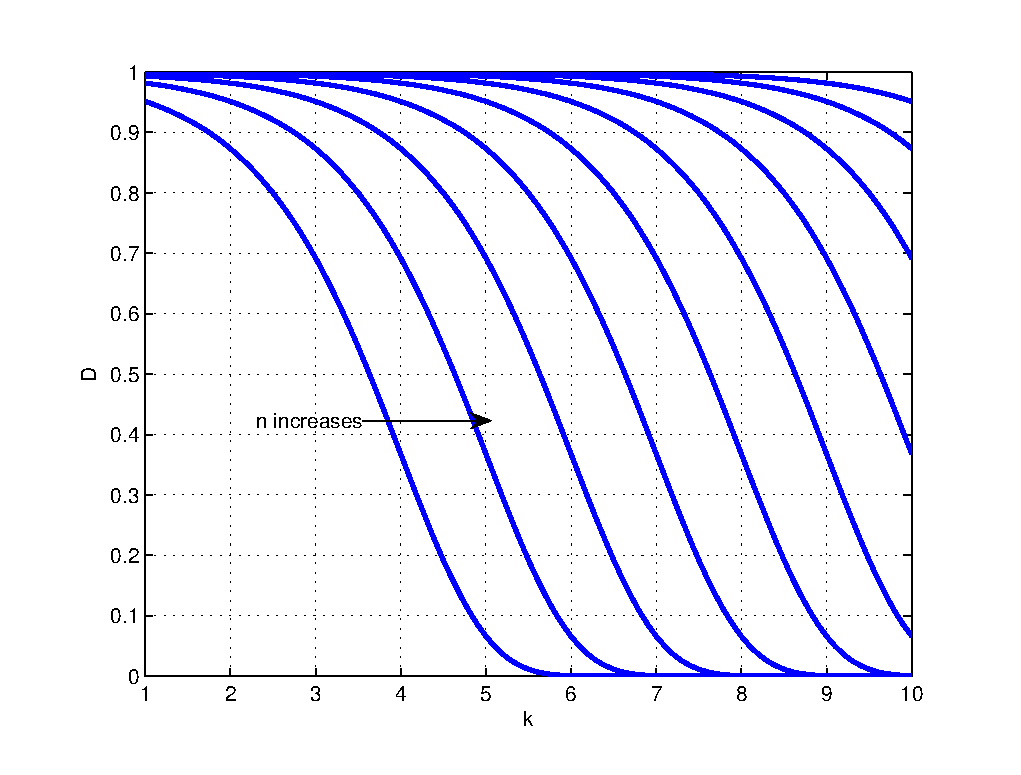
\includegraphics{democutoff1.eps}}
  \scalebox{0.5}[0.5]{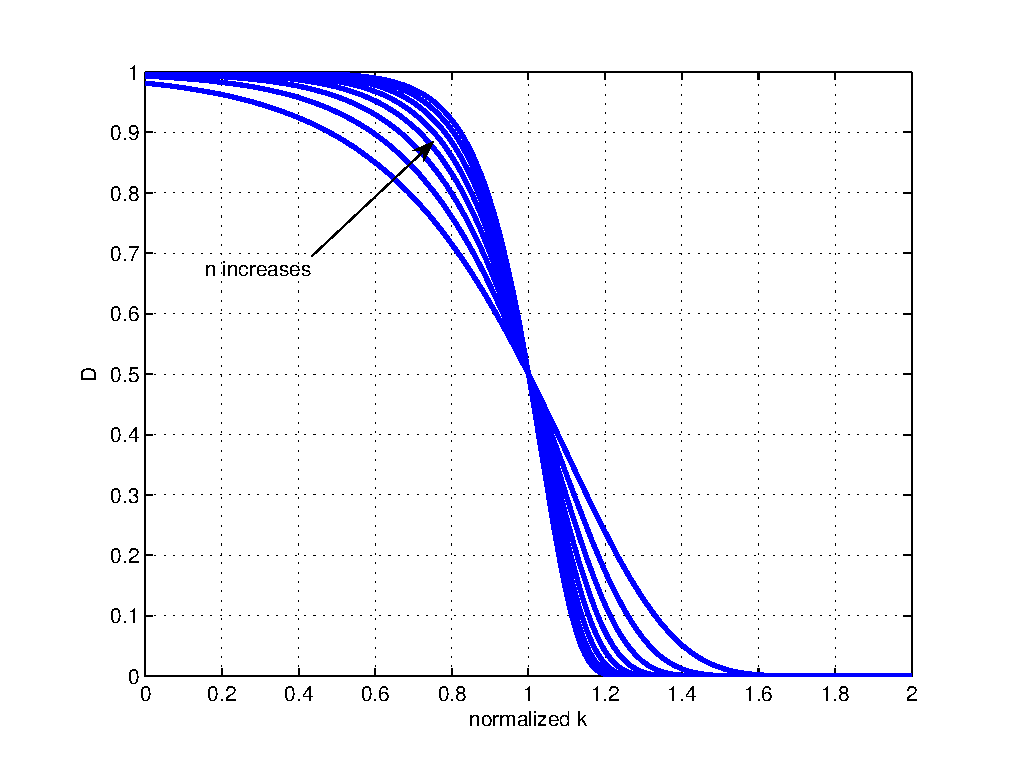
\includegraphics{democutoff1n.eps}}
} \caption{(a) A family of trajectories which present a cutoff, (b) the normalization of (a)}
  \label{democutoff1}
\end{figure}

\begin{figure}
 \centerline{
  \scalebox{0.5}[0.5]{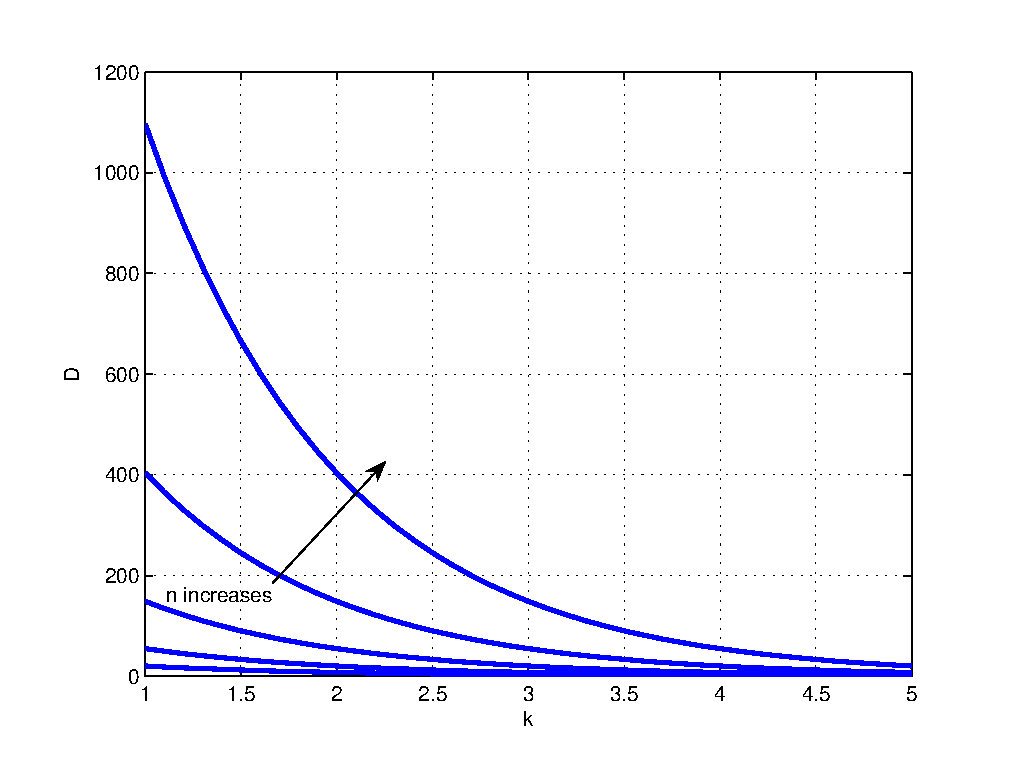
\includegraphics{democutoff2.eps}}
  \scalebox{0.5}[0.5]{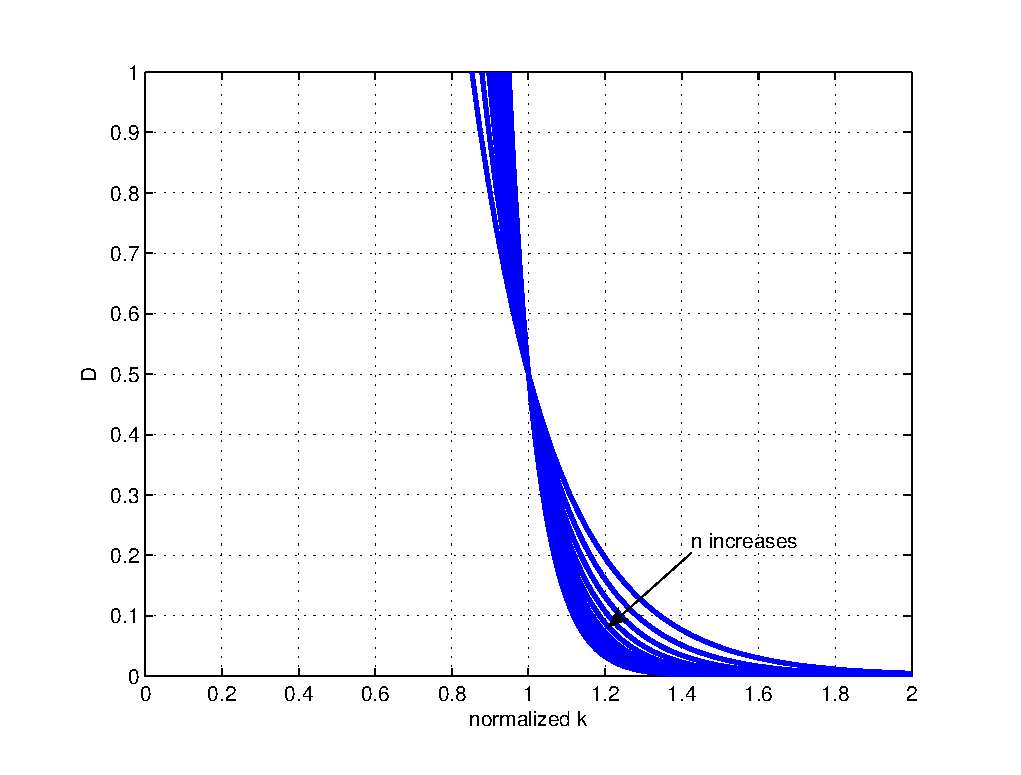
\includegraphics{democutoff2n.eps}}
} \caption{(a) A family of trajectories which present a cutoff when $D$ is unbounded above, (b) the normalization of (a)}
  \label{democutoff2}
\end{figure}


%define $\sigma: L_{T^2}^2\rightarrow \mathbb{R}$,
%\begin{eqnarray}
%[\sigma]c(\mathbf{x}) = \left(\int_{T^2}\left(  c(\mathbf{x}) -
%\bar{c} \right)^2 da\right)^{\frac{1}{2}}
%\end{eqnarray}
%where $da = dxdy$ and $\bar{c} =  \frac{\int_{T^2} c(\mathbf{x})da}{\int_{T^2}da}$ is the mean of $c(\mathbf{x})$ over
%$T^2$. $[\sigma]c(\mathbf{x})$ is equal to the $L^2$ norm of the function $c(\mathbf{x})$ when the mean of $c(\mathbf{x})$
% is zero.

%%%%%%%%%%%%%%%%%%%%%%%%%%%%%%%%%%%%%%%%%
\section{Measures for Scalar Functions and Cutoff Phenomenon}
\label{Measure for Scalar Functions}
%%%%%%%%%%%%%%%%%%%%%%%%%%%%%%%%%%%%%%%%%
\subsection{Mesaure for Chaotic Mixing}
In this section we demonstrate various norms which can be applied to measure the mixing of a scalar function. To aviod the nonzero DC term to appear in the measure, we assume all the functions have mean zero. 

Before we proceed, there are some words about the measure space. In equation (\ref{lpnorm}) and its continuous version, the measure spaces are $(\Omega, \pi)$ or $(T^2,\pi)$ and $\pi$ can be arbitrary finite or infinte measure. The choose of these measure spaces has its physical meaning and will be clear later. However, in this section, we simply let $\pi = \mathbf{1}$ as the measure to avoid the difficulty of the representation in frequency domain. Also, the goal of this section is not to compare which of these norms is better, but we want to show that the behavior of different norms can be really different. 

The candidates are the mix-norm suggested by \cite{Mezic2005}, Sobolev norms with index $s= 0$,$-0.5$, and $-1$, and a diffuse-norm we suggest. Some of these norms are much easier defined in the frequency domain. The definition of mix-norm can be found in \cite{Mezic2005}. This mix-norm is designed to resolve the inability of the $L^2$ norm to capture small-scale
(high frequency) variations when advected by chaotic maps without diffusion. However, it is also a good measure when diffusivity exists.  

 
Here the definitions of other norms in frequency domain are given. For a function $c \in L^{2}_{T^2}$, which has a Fourier representation $c(\mathbf{x}) = \sum_{k \in \mathbb{Z}^n} a_\mathbf{k} e^{i 2 \pi \mathbf{k.x}}$, where $\mathbf{k}=\sqrt{k_1^2+k_2^2}$ and $k_1$ and $k_2$ are the wave number on $x_1$ and $x_2$ directions. The Sobolev norm $H^s$ is given by,
\begin{eqnarray}
  \|c\|_{H^s} = \sqrt{\sum_{k \in \mathbb{Z}^n}   \left(1+(2 \pi \|\mathbf{k}\|)^2\right)^s |a_{\mathbf{k}} |^2   }
\end{eqnarray}

The diffuse-norm $\|\cdot\|_D$ is
\begin{eqnarray}
  \|c\|_D = \sqrt{\sum_{k \in \mathbb{Z}^n} e^{-4 \pi^2 D \|\mathbf{k}\|^2} |a_{\mathbf{k}} |^2   }
\end{eqnarray}
Physically, the diffuse-norm is equivalent to diffuse the function $c$ with the diffusivity rate $D$ for one unit time step and then measure the $L^2$ norm. So it can be also written as,
\begin{eqnarray}
  \|c\|_D = \|[M(D,1)] c \|_{H^0}
\end{eqnarray}
Hence all these norms are different only on the coefficient multiplied by $|a_{\mathbf{k}} |^2$. We thus plot these coefficients as a function of $\mathbf{k}$ in figure \ref{normcompare}

\begin{figure}
\caption{\label{normcompare} Weights on different wave numbers for different norms}
\centerline{\scalebox{0.5}[0.5]{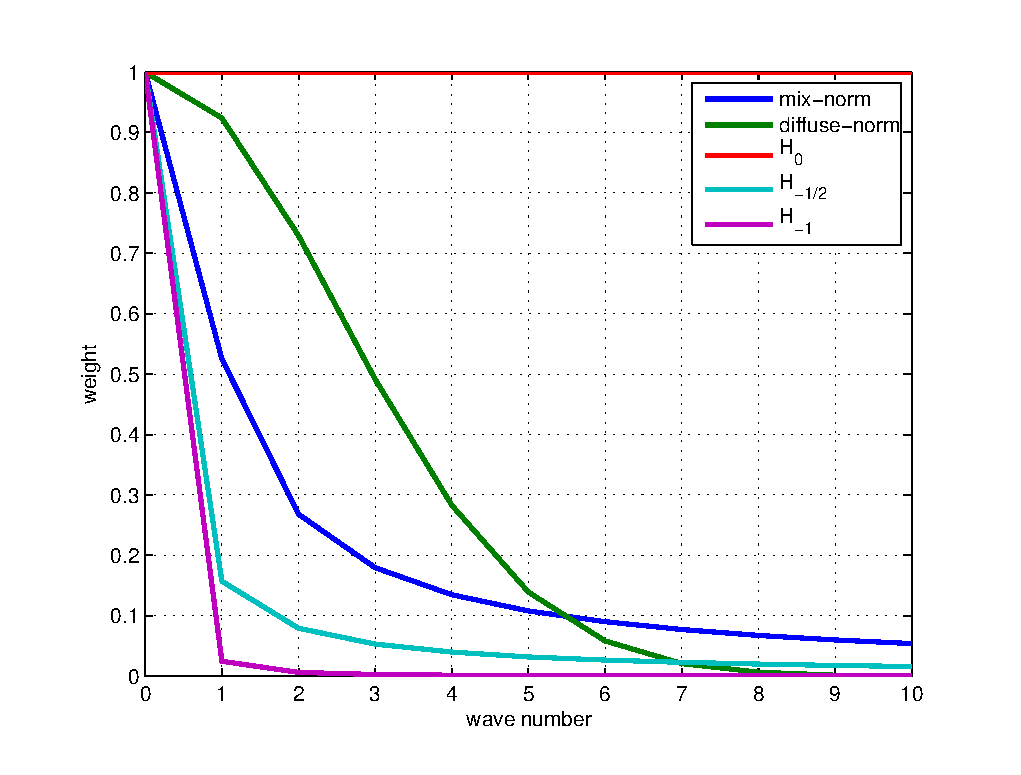
\includegraphics{normcompare.eps} }}
\end{figure}

In figures \ref{normplot} and \ref{lognormplot} we show the simulations of standard map with the chaotic parameter $\epsilon =0.2$, diffusivity rate $D = 1e-5$ and initial condition $\mathbf{x} = cos(x)$. All norms capture the increase of mixing successfully, whereas the details are different. $L^1$ and $H_0$ (which is just $L^2$) norms decay super-exponentially and have concave shapes before iteration $20$. The other norms drop fast in the beginning. In \cite{Mezic2005} the author claims that the mix-norm is equivalent to $H_{-\frac{1}{2}}$ norm. This fact is clearly shown in this simulation. One should also notice that the diffuse-norm has very similar tendency with the above two norms. This result is not surprising because in figure \ref{normcompare} they all have monotonic decreasing weights on high wave numbers.

\begin{figure}
\caption{\label{normplot} The norm-iteration plot of standard map with diffusivity rate $D = 1e-5$}
\centerline{\scalebox{0.5}[0.5]{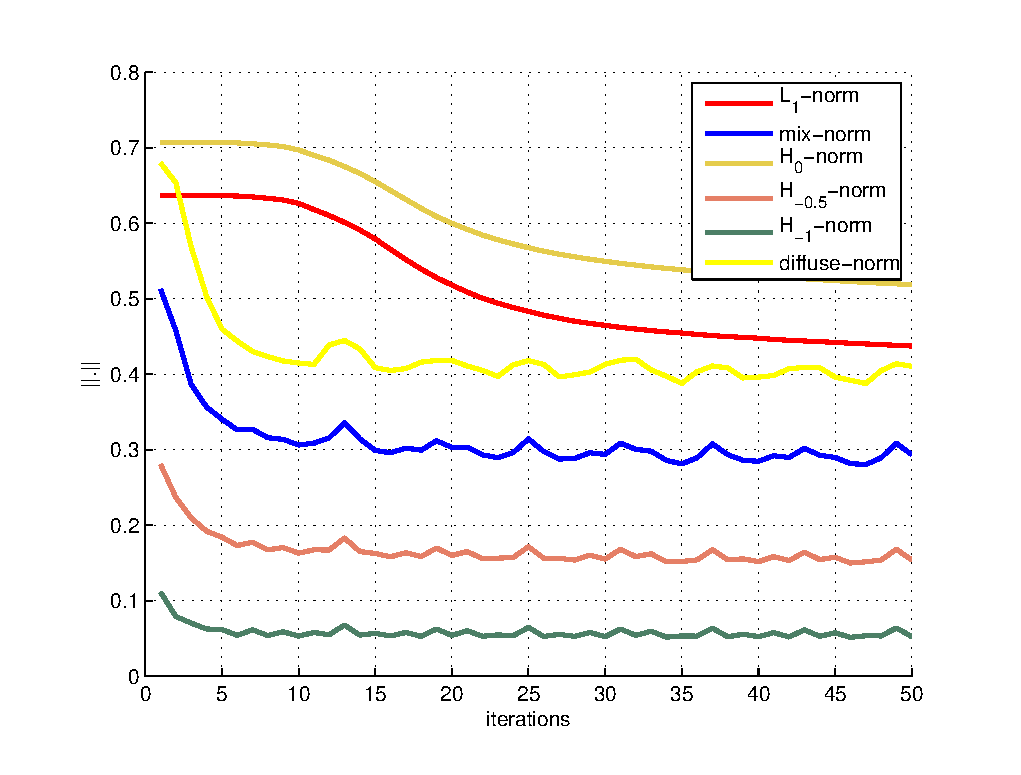
\includegraphics{normplot.eps} }}
\end{figure}
\begin{figure}
\caption{\label{lognormplot} The norm-iteration log plot of standard map with diffusivity rate $D = 1e-5$}
\centerline{\scalebox{0.5}[0.5]{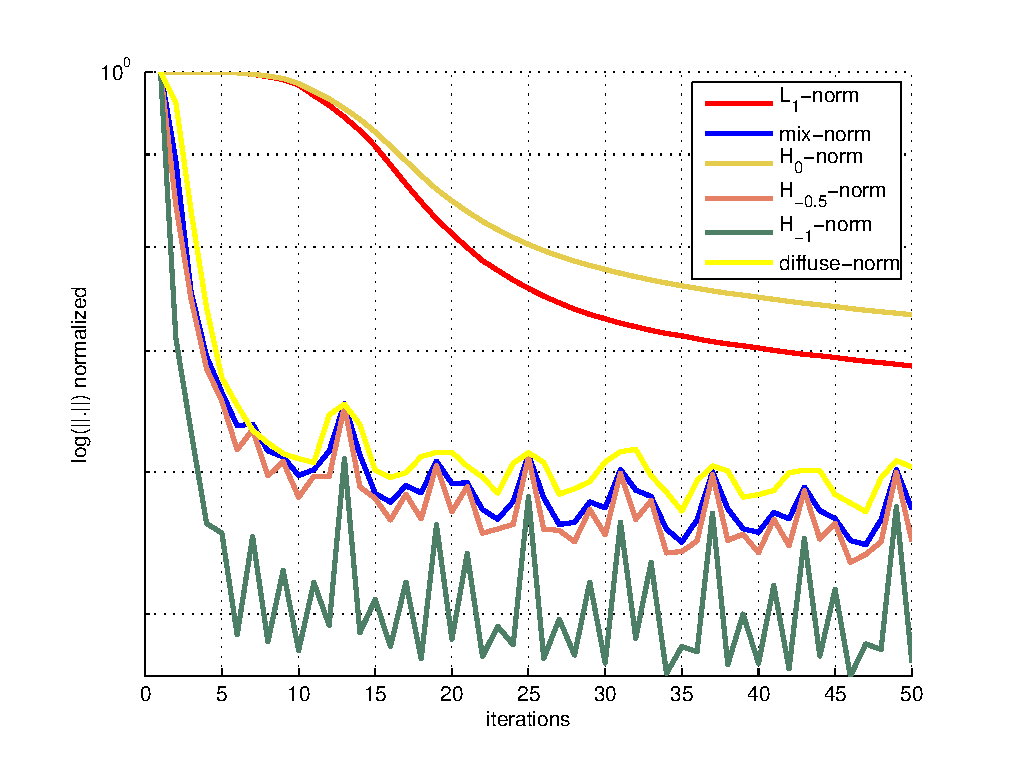
\includegraphics{lognormplot.eps} }}
\end{figure}



We think all the norms discussed above are valid for measuring the chaotic mixing of a scalar function. Which norm one should apply is dependent of what one cares the most. In later sections we will discuss the super-exponential decays observed in $L^1$ and $L^2$ measures. They are mainly due to the weights in high wave number terms. 




%%%%%%%%%%%%%%%%%%%%%%%%%%%%%%%%%%%%%%%%%
\section{The Markov Chain Model of a Map}
\label{The Markov Chain Model of a Map}
%%%%%%%%%%%%%%%%%%%%%%%%%%%%%%%%%%%%%%%%%
In the rest of this paper, we focus on the properties of the advection-diffusion operator $[P(D,1)]$, i.e. the Frobenious-Perron operator for a given map $S$ with diffusivity $D$. A sparse Markov chain model is proposed to approximate it. Numerically, the diffusion can be added easily in frequency domain. So the simplest way to obtain $[P(D,1)]$ is to use (\ref{PDdef}), and then approximate by a finite dimensional operator. However, the operator one obtains is essentially a full matrix and thus hard to operate efficiently. We would like to use an alternative way to approximate $[P(D,1)]$, the operator we get is extremely sparse and easy to evolve. Similar approaches can be found in, for example \cite{Pierrehumbert2000}\cite{Tsang2005} and is called lattice method. However, here we emphasis the procdeure to obtain a sequence of Markov chain models with decreasing numerical diffusion and increasing accuracy. 




The idea behind this procedure is that a Markov chain is intrinsically diffusive, and when we use a Markov matrix $P_h$ to
approximate the non-diffusive $[P]$, a small numerical diffusion has been added inevitably. This numerical diffusion decreases when a higher resolution model is applied. Thus we can form a sequence of Markov chain models of the same system with decreasing numerical diffusion.  


In large scale (the scale much larger than the grid size $h$), the numerical diffusion induced by modeling behaves like the physical diffusion, i.e. the $D(u_{xx}+u_{yy})$ term in (\ref{advection-diffusion equation}). However, this similarity usually breaks down in high wave numbers. This is also the reason any numerical scheme is only valid to simulate a physical system below certain frequency. When talking about simulations of chaotic maps, the frequncy bound is really a problem. This is because the frequency cascade of chaotic maps makes the system touch this frequency bound in just several iterations, and even tiny diffusion could affect the system behavior in high frequency. Hence no good strategy has been suggested to simulate chaotic systems with exponentially growing high frequency terms. This frequency bound can also be improved by using higher-order accuracy methods, but these methods are usually nonlinear and beyond the scope of this paper.  

In spite of the discrepancy of the difference of the numerical diffusion and the phyiscal diffusion in high frequency terms, our model does show the tendency of the chaotic system behavior when diffusion is reducing, and it is consistent with other methods which solve (\ref{advection-diffusion equation}) in lower resolution.  
    


\subsection{The Choice of Frobenious-Perron Operator}

We would like to find a finite dimensional approximation of the Frobenious-Perron Operator for a map $S$. The strategy is to first approximate it by the finite Markov operator, and then use (\ref{fevolve}) to evolve the system.

We discretilize the domain $T^2$ into $1/h$ by $1/h$ regular grids, and thus a probability measure $\mu$ on $T^2$ is represented by $\mu_h = [d_h]\mu$, i.e. a distribution with $1/h^2$ states. For a finite $h$ this is of course just an approximation. Now we want to choose Markov matrices $P_h^+$ and $P_h^-$ to achieve
 \begin{eqnarray}
 (P_h^+)^T [d_h]\mu = [d_h]S(\mu)\\
 (P_h^-)^T [d_h]\mu = [d_h]S^{-1}(\mu) \nonumber
 \end{eqnarray}
for any $\mu$. Such $(P_h^+)$ and $(P_h^-)$ may not exist for finite $1/h$. The natural choice for them are the following,
 \begin{eqnarray}
 (P_h^+)^T = [d_h]S[d_h]^\dagger \\
 (P_h^-)^T = [d_h]S^{-1}[d_h]^\dagger \nonumber
 \end{eqnarray}
where $[d_h]^\dagger$ is one of the pseudo-inverse of $[d_h]$.
 \begin{eqnarray}
 [d_h]^\dagger = [N][d_h]^T([d_h][N][d_h]^T)^{-1}
 \end{eqnarray}
and $[N]: T^2 \rightarrow T^2$ is an operator one can choose freely. Our choice is $[N]=[N_{\pi}] = \text{diag}(\pi)$, i.e. it multiplies a distribution by $\pi$ point-wise, where $\pi$ is one of the invariant distribution of $S$. This makes
\begin{eqnarray}
  (P_h^+)^T \pi_h =  \pi_h \\
  (P_h^-)^T \pi_h =  \pi_h \nonumber
\end{eqnarray}
i.e. $ \pi_h =[d_h]\pi$ is the left eigenvector of both $P_h^+$ and $P_h^-$ corresponding to the eigenvalue $1$. This choice ensures both of the Markov chains converge to the invariant distribution we choose, and $(P_h^+)^* = P_h^-$, i.e., they are a pair of adjoint operators.

More explicitly, one can calculate $P_h^+$ and $P_h^-$ by
\begin{eqnarray}
\label{P definition}
     (P_h^+)_{ij} = \frac{\int_{S(a_i) \cap a_j  } \pi(\mathbf{x})da}{\int_{a_i} \pi(\mathbf{x}) da
     } \mbox{   , for all } i,j\\
     (P_h^-)_{ij} = \frac{\int_{S^{-1}(a_i) \cap a_j  } \pi(\mathbf{x})da}{\int_{a_i} \pi(\mathbf{x}) da \nonumber
     } \mbox{   , for all } i,j
\end{eqnarray}
Then from (\ref{fevolve}), we know $P_h =(P_h^+)^* = P_h^-$ is the matrix to evolve a function forward in time, and hence the
approximation of the Frobenious-Perron operator. Note that it is no difference between finding $P_h^-$ directly or finding the adjoint operator of $P_h^+$ if $\pi$ is known. However, it is possible that $\pi$ is found numerically and not very accurate. In such case, finding $P_h^-$ directly would be a preferable idea. We will discuss this later.

\subsection{The Choice of $\pi$}

The above setting has a very nice physical interpretation when the map $S$ comes from a periodical mixing channel. In that case, the fluid particle is transported by the map, and the scalar function represents the color which a particle carries. The natural choice of the invariant distribution $\pi$ is the velocity distribution normal to the cross section of the channel when the flow is stationary. If one observes the color at the cross section every period of the channel, the total color (sum of $f$) does not keep constant, but the total color flows in and out per unit time have to be the same, i.e.
$(f^k)^T\pi =(f^{k+1})^T\pi$, due to the mass conservation. 

However, such a natural choice of $\pi$ may not exist for a general chaotic map. There are infinite number of invariant distributions. For example, in the simulation of standard map figure (\ref{standardmapdotplot}), each of the small orbit has a corresponding invariant distribution if we assign equal probability on it and zero elsewhere, but these are obviously not the one we want. The specific invariant distribution $\pi$ and the Markov matrix $P_h$ we use satisfy the following three conditions,

\begin{enumerate}
\label{invariant equation}
 \item $\pi = S(\pi)$
 \item $\pi_h= P_h^T \pi_h$
 \item $P_h$ is irreducible.
\end{enumerate}

The irreducibility of $P_h$ ensures that every state can access every other state through some path. Therefore the state is diffusive and cannot have any zero entry in $\pi_h$. The three conditions certainly eliminate most of the unwanted stationary distribution, but it does not tell us how to find such a distribution. Here is our rule of thumb:
\begin{itemize}
  \item If the map comes from a physical system, usually one has a
  natural choice like the velocity distribution in the flow channel case.
  \item If the map is volume-preserved, then uniform distribution is
  obviously an invariant distribution satisfying the three
  conditions.
  \item For other cases, a bin method is applied. one can simulate the map with a set of randomly
  distributed points, accumulates the mapped points at each bin until it converges to
  an invariant distribution. The bin size is selected to be $h$. 
\end{itemize}

 


\subsection{Numerical Strategy}
In reality, none of the two equations in (\ref{P definition}) is achievable because of the high cost of numerical integration of $S(a_i) \cap a_j$ or $S^{-1}(a_i) \cap a_j$. Hence a further simplification needs to be done. In our simulations, in stead of mapping the region $a_i$ backward and finding the intersection with all $a_j$s to set the weightings, we only map the four corners of the $a_i$ grid back and find which $a_j$ they belong, and set the nonzeros to be $1/4$. That is, let $\mathbf{x}_i=(x_{1i},x_{2i})$ be the center of grid $a_i$,
 \begin{eqnarray}
   (\hat{P_h})_{ij} =\left\{ \begin{array}{cc}
                     \frac{1}{4} &\mbox{, if } S^{-1}(x_{1i}\pm \frac{h}{2},x_{2i}\pm \frac{h}{2}) \in a_j \\
                     0          &\mbox{, else} \\
                     \end{array} \right.              
 \end{eqnarray}
This method is silmiliar to the lattice method used in \cite{Tsang2005}\cite{Pierrehumbert2000}. However, the lattice method maps the center of the grid $a_i$ backward and uses a linear interpolation to find this off-grid value. The numerical diffusion is thus created by the linear interppolation step, and it happens BEFORE mapping. Our approach creates the numerical diffusion when averaging the four corners, and hence it happens AFTER mapping. 

This numerical strategy is extremely simple and can be implemented and computed in parallel without any difficulty. However, it only captures part of the features of (\ref{P definition}). The major differences are: firstly, the stationary distribution $\pi(\mathbf{x})$ inside the integration is ommited because only four nonzeros are selected in each row so that there is no way to put correct weights, and which are the key to ensure the largest left eigenvector of $P_h$ to be $\pi_h$. However, it is clear that when the grid size gets smaller, the weight $\pi(\mathbf{x})$ in (\ref{P definition}) becomes less important, and the Markov chain should still have the correct invariant distribution in the limit case. One can tell whether the grid size is small enough by comparing $\pi_h$ and the stationary distribution of $\hat{P_h}$. In all of our simulations, when $1/h$ is larger than several hundreds, they agree well. 
Secondly, there are at most four nonzeros in each row of $\hat{P_h}$, but apprently there could be more in $P_h$. The four nonzeros in each row of $\hat{P_h}$ may not even be connected in space if the map stretches this grid a lot. Nonetheless, this discrepancy also become insignificant when grid size tends to zero, because in this case a map cannot stretch a grid too much. In fact, one can show that $P_h$ and $\hat{P_h}$ are both first order accuracy to the original map $S$, just with a different constant multiplying the error. One should also be noted that setting the weights to be all equal is not an approximation if at the previous step the function is defined as a piecewise constant one on grids. 


\subsection{Additional Smoothing Step}
Using the numerical strategy in the previous section, we can simulate the map with some small numerical diffusion. The effect of numerical diffusion is similar to physical diffusion in large scale, but their behaviors can be quite different in small scale, and these small scale phenomenon might be quite important for a chaotic map to form its stationary eigen direction. Therefore to simulate the physical diffusion correctly, we need to simulate the map with far higher resolution with some additional diffusion terms. The additional smoothing step can be added by either in spatial or frequency domain. In spatial domain, we adopt the method used in [\cite{Tsang2005}], 
 \begin{eqnarray}
   f^{k+1}_{(p,q)} = \sum_{|r|,|s|\le 2}C_{|r|}C_{|s|}f^{k+1}_{(p,q)}
 \end{eqnarray}
Which creates a large scale diffusion $D=h^2$. In frequency domain, a two dimensional FFT/IFFT with a multiplication of a constant between them according to the wave numbers can be applied. 

%The following figure shows some simulation results. The map we use is Standard map. Figure [x] shows the power spectra at first 30 iteration without any additional smoothing step. The grid size $h= 1/80000$. One can observe the pileup in the high wave number terms during 10 to 20 iterations. Comparing this with the 2-norm plot on the right hand side, it shows a super-exponential decay between 10 and 20 iterations. 

%Figure [x] we compare the spatial and frequency domain smoothing strategies. The red and green lines show the map at its 1 to 8 iterations with spatial and frequency smoothing after each step, respectively. The grid size here is also $h= 1/80000$. Both cases eliminate the pileup and they are almost the same at low wave number terms. The discrepancy in high wave number terms can of course affect the stationary decay rate ...


     

 
    


\subsection{Simulations}

The following three figures are to demonstrate the feasibility of the Markov model. In figure \ref{standardmapdotplot} a set of random points in $T^2$ are evolved by standard map with $\epsilon=0.2$ for 300 iterations. The locations of these points after every iteration are plotted. One can clearly observe it forms many small orbits in some region. Figure \ref{standardmapsimuexact} shows the final distribution when $c(x,y) = \cos(x)$ is evolved by the Frobenious-Perron operator for 40 iterations. Because $\cos(\cdot)$ is an analytical function, this can be done exactly by the inverse map $S^{-1}$. Some islands are clearly formed and for the other region the color is completely random. Figure \ref{standardmapsimumarkov} then shows the same simulation performed by the Markov matrix $P_h$ with number of grids $1000$ by $1000$. As we have mentioned above, there are some inevitable diffusion in the Markov model, the color in the "random" region are mixed. The
diffusion is so small so the "island" region is well formed. $P_h$ has nonzero density $4.03\%$, $\text{nnz} =4027356$, so it is very sparse.


\begin{figure}
\caption{\label{standardmapdotplot} A set of random points evolved
by standard map with $\epsilon=0.2$}
\centerline{\scalebox{0.5}[0.5]{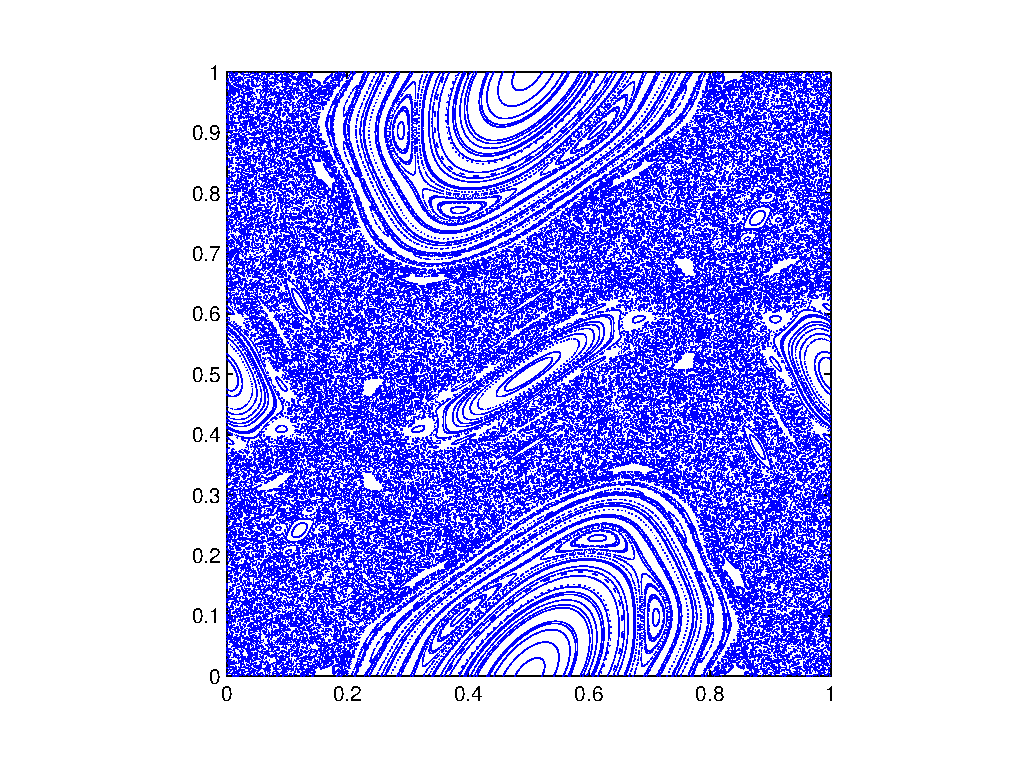
\includegraphics{standardmapdotplot.eps}}}
\end{figure}

%\begin{figure}
%\caption{\label{standardmapsimuexact} $\text{cos}(x)$ function
%evolved by standard map for 40 iterations}
%\centerline{\scalebox{0.5}[0.5]{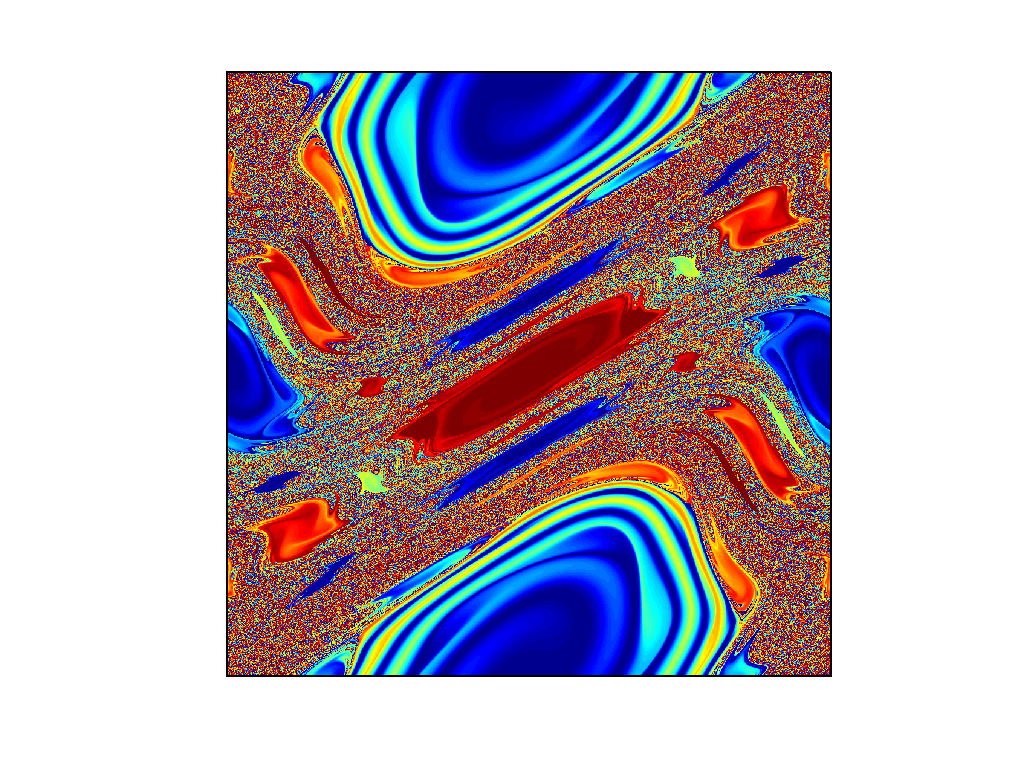
\includegraphics{standardmapsimuexact.eps}}}
%\end{figure}

%\begin{figure}
%\caption{\label{standardmapsimumarkov} $\text{cos}(x)$ function
%evolved by the Markov chain model of standard map for 40 iterations
%}
%\centerline{\scalebox{0.5}[0.5]{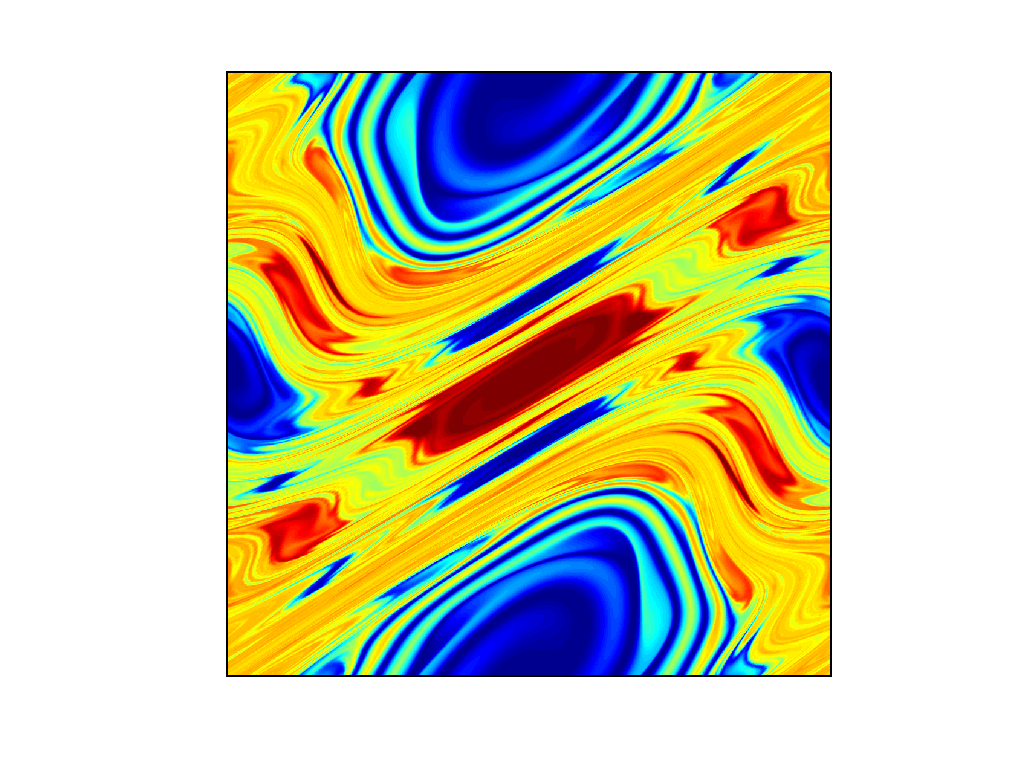
\includegraphics{standardmapsimumarkov.eps}}}
%\end{figure}


\begin{figure}
\centerline{
\scalebox{0.5}[0.5]{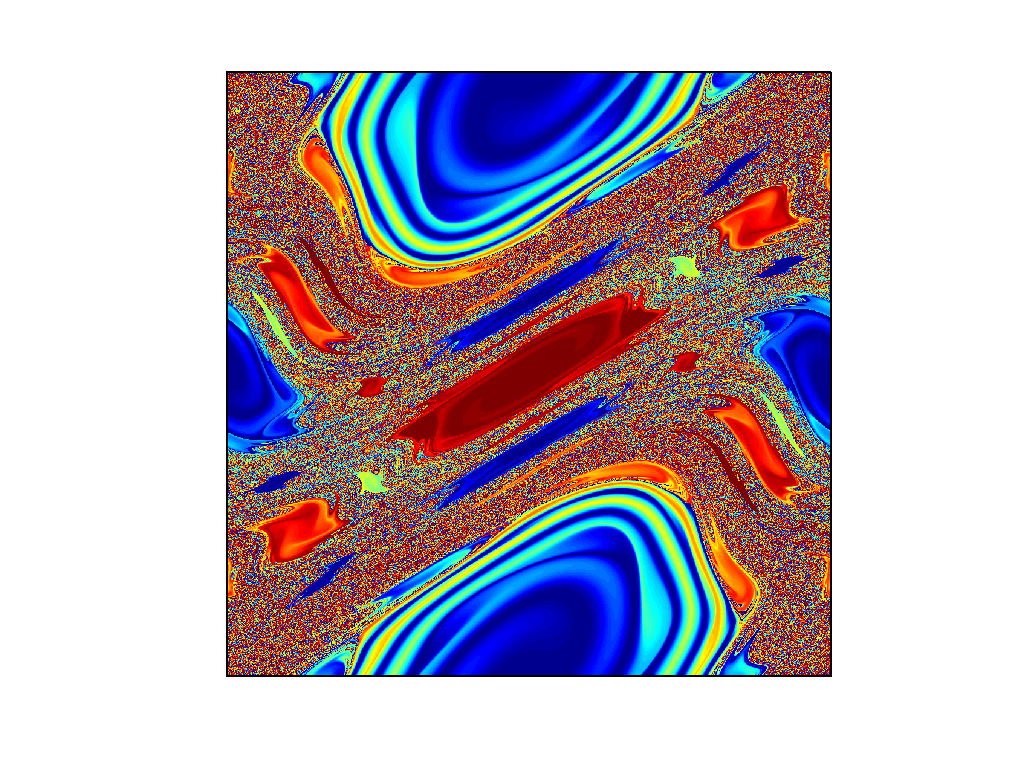
\includegraphics{standardmapsimuexact.eps}}
\scalebox{0.5}[0.5]{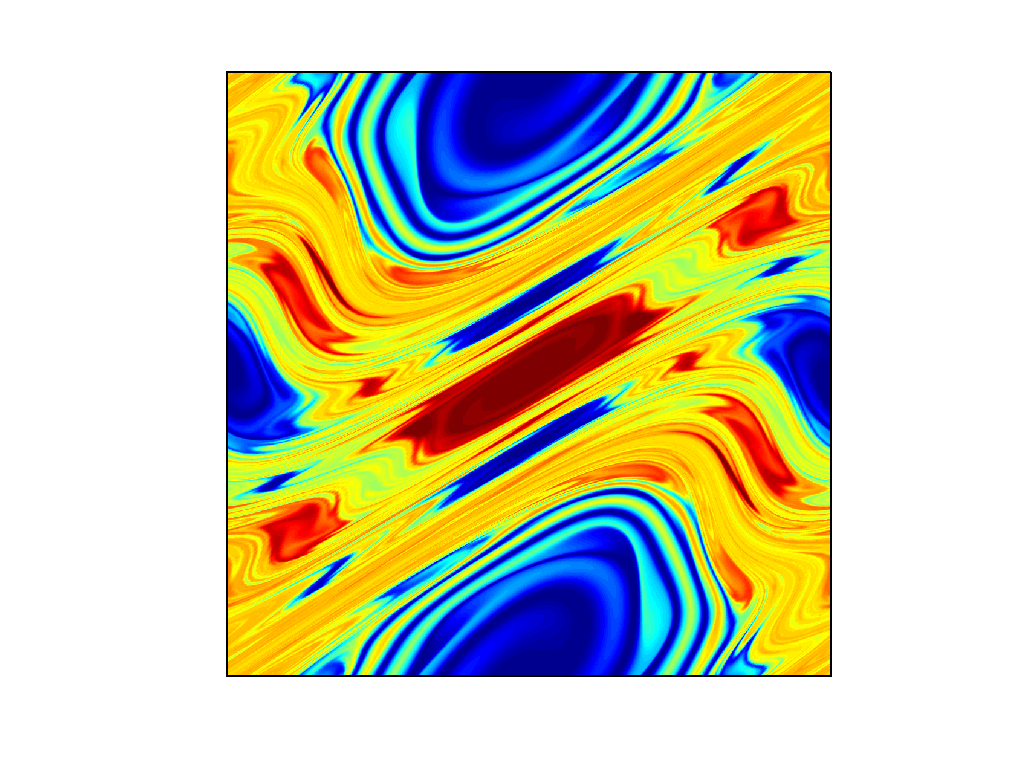
\includegraphics{standardmapsimumarkov.eps}} }
\caption{\label{standardmapsimuexact}  $\text{cos}(x)$ function
evolved by standard map for 40 iterations}
\caption{\label{standardmapsimumarkov} $\text{cos}(x)$ function
evolved by the Markov chain model of standard map for 40 iterations}
\end{figure}


The Markov model will serve as our main tool to study the effect when more diffusion is added to the map. Thus before we do that, we should first justify how large the diffusivity rate is for the
Markov model.





%%%%%%%%%%%%%%%%%%%%%%%%%%%%%%%%%%
\section{The Cut-off Phenomenon of Chaotic Mixing Processes}
\label{The Cut-off Phenomenon of Chaotic Mixing Processes}
%%%%%%%%%%%%%%%%%%%%%%%%%%%%%%%%%%
In many Markov chian simulations, one can observe a 2 or 3-stage convergence rate change just like we see in the advection-diffusion equation simulations. This phenomenon is named cutoff. For linear systems like Markov chains, eigen-structure analysis is probably the most powerful tool to study how cutoff happens. Nonetheless, it shows less physical reason of why a system has cutoff. On the other hand, people have studied a similiar multi-stage chage and linked it to the physical mixing property of advection-diffusion operators of various chaotic maps. We think these two fields are tightly related. More percisely, the cutoff phenomenon of a linear system is actually an imitation of the nonlinear behavior of some chaotic systems.


It is noticed that for some of the Markov chains which have cutoffs, the rate of convergence before the exponentional decay
region is doubly exponentional. So let us begin with a function which decays doubly exponentinally. Consider the following sequence,
 \begin{eqnarray}
 \label{doublyconvergence}
 \varphi^k_n = \text{e}^{-a^{k-n}}
 \end{eqnarray}

where $a>0$ is a real number. It is easy to see that if $D(\mu^k_n,\nu_n)=\varphi^k_n$, the family $(\Omega_n,\nu_n, (\mu^k_n)_{k=0,1,...})_{n=1,2,...}$ satisfies the definition of cutoff. If one ask the question: what kind of linear system family has the above congergence property? The answer is not obvious at all. However one can easily find a family of nonlinear advection-diffusion operators with varying diffucivity rate which possess this convergence feature. Consider the following examples,

\begin{example}
Consider the homogeneous baker's map on $T^2$,
  \begin{eqnarray}
    S(x_1,x_2) =  \left\{ \begin{array}{cc}
                 (2x_1,\frac{1}{2}x_2) \mbox{ mod } 1      &\mbox{, if } 0\le x_1 < \frac{1}{2} \\
                 (2x_1,\frac{1}{2}(x_2+1)) \mbox{ mod } 1  &\mbox{, if } \frac{1}{2}\le x_1< 1\\
              \end{array} \right.
  \end{eqnarray}
with initial condition $c^0(\mathbf{x})= \pi^{\frac{1}{2}}\cos(2 \pi
x_2)$, diffusion operator with diffucivity $D$ is applied after every iteration. The problem is analytical solvable, and we have,
  \begin{eqnarray}
   c^l(\mathbf{x}) = \pi^{\frac{1}{2}}\text{e}^{-4 \pi^2 D 2 ^{2 l}}\cos(2 \pi 2^l
   y) \mbox{ for }l = 1,2,...
  \end{eqnarray}
and the 2-norm of $c^l(\mathbf{x})$ is
  \begin{eqnarray}
  \label{bakersmapconvergence}
   \|c^l(\mathbf{x})\|_2 = \text{e}^{-4 \pi^2 D 2 ^{2 l}}
  \end{eqnarray}
Comparing (\ref{bakersmapconvergence}) with
(\ref{doublyconvergence}), if let $l=k$, $a=4$ and $D =\frac{4^{-n-1}}{\pi^2}$,
one can certainly build the convergence sequence.
\end{example}
%%%%%%%%%%%%%%%%%%%%%%%%%%%%%%%%%%%%%%%%%%%%%%%%%%%%%%%%%%%%%%%%%%%%%%%%%%%%%%%%%%%
%In fact a even simpler map can achieve this,
%\begin{example}
%Consider Arnold's cat map on $T^2$,
%  \begin{eqnarray}
%               x_1' \leftarrow  2x_1+x_2 (\mbox{ mod } 1)\\
%               x_2' \leftarrow  x_1+x_2 (\mbox{ mod } 1) \nonumber
%  \end{eqnarray}
%with initial condition and diffusion the same as the previous
%example. The map maps wave number in $x_1$ and $x_2$ directions as
%  \begin{eqnarray}
%  \label{wavenumberexp}
%    \left[\begin{array}{c}
%           k_1'\\
%           k_2'
%    \end{array}\right] =
%    \left[\begin{array}{cc}
%           1& -1\\
%           -1& 2
%    \end{array}\right]
%    \left[\begin{array}{c}
%           k_1\\
%           k_2
%    \end{array}\right]
%               %k_1' &=& k_1  - k_2 \\
%               %k_2' &=& -k_1 + 2 k_2  \nonumber
%  \end{eqnarray}
%One can easily check that the magnitude of the wave number $(k_1,k_2)$ in (\ref{wavenumberexp}) grows exponentionally. Hence similiar to the Baker's map example, the doubly exponentioal decay sequence can be easily built.
%\end{example}

The above example shows that we can create a family of advection-diffusion operators with indices $n$ which presents a
"cutoff". If we apply the modeling procedures disscussed in section \ref{The Markov Chain Model of a Map} and \ref{A Frequency Domain Approach} to the above examples, and the grid size $h$ is small enough to capture the doubly exponential convergence corrcectly up to $\tau^D_n$ , we can surly get the corresponding finite dimensional linear map which satisfies the first condition of the definition of a cutoff. Because it is just a finite dimensional linear model, finally the state has to evolve to one of its eigenvector direction, and then the norm decays exponentially. This exponential decay region is due to the resolution of the model and has nothing to do with the original system. Hence the second condition is not guarenteed to be satisfied. 

%On the other hand, for some of the chaotic maps like standard map, a persistant pattern is formed after a number of iterstions when finite diffusivity exists. This is the so-called strange eigen-mode. It has been discussed widely about whether the decay rate at this region tending to a constant independent of $D$. In the simulations given we had done, we see that for standard map, it does converge to a constant, and clearly, this makes the second condition of a cutoff satisfied. 






To be more percise, let us first extend the definition of a cutoff to the continuous space $T^2$. Assume that, any
pair of probability measures $\mu$, $\nu$ on $T^2$ is associated
a real number $D(\mu,\nu)$ such that $D(\mu,\nu)\in [0,1]$,

\begin{eqnarray}
\max_{\Omega,\mu,\nu} D(\mu,\nu) = 1
\end{eqnarray}
and $D(\mu,\nu)=0$ if and only if $\mu=\nu$. Consider a sequence of
probability measures $\nu_n$ on $T^2$, $n=1,2,...$, each
equipped with a sequence of probability measure $\mu^k_n$,
$l=0,1,...$, such that
\begin{eqnarray}
\lim_{k \rightarrow \infty} D(\mu^k_n,\nu_n)=0
\end{eqnarray}
The definition of a cut-off is,
\begin{definition}
\label{cutoffdefition}
A family $(T^2,(\nu_n, (\mu^k_n)_{k=0,1,...})_{n=1,2,...})$
presents a D-cut-off if there exists a sequence $(t_n)$ of positive
reals such that, for any $\epsilon \in(0,1)$,
\begin{enumerate}
  \item $\lim_{k \rightarrow \infty}D(\mu^{k_n}_n,\nu_n) = 0 \mbox{ if }
  k_n>(1+\epsilon)t_n$
  \item $\lim_{k \rightarrow \infty}D(\mu^{k_n}_n,\nu_n) = 1 \mbox{ if }
  k_n<(1-\epsilon)t_n $
\end{enumerate}
\end{definition}

The above definition is nothing more than changing all the finite probability spaces $\Omega_n$ in definition 1 to a continuous one $T^2$. Now we state the relation between the two definitions.

\begin{theorem}
suppose the family $(T^2,(\nu_n,(\mu_n^k)_{k=0,1,...})_{n=1,2,...})$ presents a D-cutoff in the sense of definition 2, then there exists a sequence $1/h_n$ of positive integers such that $(\bar{\Omega}_n,\bar{\nu}_n,(\bar{\mu}_n^k)_{k=0,1,...} )_{n=1,2,...}$ presents a $\bar{\text{D}}$-cutoff in the sense of definition 1, where 
\begin{eqnarray}
      \bar{\nu}_n &=& [d_{h_n}]\nu_n\\
      \bar{\mu}_n^k &=& [d_{h_n}]\mu_n^k\\
      \bar{\Omega}_n &=& \{ a_1,a_2,...,a_{1/{h_n^2}} \}\\
      \bar{D}(\bar{\nu},\bar{\mu})&\equiv& D([d_{h_n}]^\dagger\bar{\nu}_n,[d_{h_n}]^\dagger \bar{\mu}_n)  
\end{eqnarray}  
\end{theorem}

\paragraph{Proof}
 \begin{eqnarray}
  \lim_{h \rightarrow 0} | D(\nu_n,\mu_n) - D([d_{h_n}]^\dagger\bar{\nu}_n,[d_{h_n}]^\dagger \bar{\mu}_n)  |=0
 \end{eqnarray}

Therefore a sequence of systems with cutoff in the sense of definition 2 implies a $(\bar{\Omega}_n,\bar{\nu}_n,(\bar{\mu}_n^k)_{k=0,1,...} )_{n=1,2,...}$ which presents a D-cutoff, but this is not saying such a sequence of Markov chains exist. In fact, the modeling procedure we present in previous section generates such a Markov chain sequence automatically. 


%%%%%%%%%%%%%%%%%%%%%%%%%%%%%%
%\subsection{Cutoff and Mixing}
%\label{Cutoff and Mixing}
%%%%%%%%%%%%%%%%%%%%%%%%%%%%%%
%The above results suggest a strong relation between the cutoff phenomenon and the mixing process of a chaotic map. A natrual question arised here is: are there any examples which have both probability and chaotic mixing interpretations? The answer is not known now. Here we try our best to grab the hints we have.

%\paragraph{Initial Condition Issue}
%In all of the mixing examples we use a  $c^0(\mathbf{x})= \pi^{\frac{1}{2}}\cos(2 \pi x_2)$ as the initial condition. According to the $\ell^p$ norm definition, this function has the same norm no matter what grid size one chooses to descretlize it. This makes the sequence of markov chains we get always has an upper bound in its norm regardless of $p=1$ or $2$. On the other hand, in most of the probability examples which present cutoffs, this is not true. Let us take the random walk on a hyper cube problem, the initial state is always equal to $[1,0,0,...0] \in \mathbb{R}^{2^n}$ which has an increasing distance to the stationary distribution $[\frac{1}{2^n},\frac{1}{2^n},...,\frac{1}{2^n}]$ when $\ell^2$ norm is applied, and one needs to use the generalized definition of cutoff (make the upper bound 1 to $\infty$). We shall point out this discrepancy may be because of the coordinate one use to describe the system. We can simply represent the mixing example in frequency domain, and then the initial conditions of the sequence of Markov chains would be exactly the same as the random walk problem with some permutation since $c^0$ contains only a single frequency. 



       









A cutoff means the distance to stationary stays high for a while and then drops
to it rapidly. If we use the this kind of map as a mixing protocol, an optimal
number of iterations can be certainly found.

However, in the above two examples, the magnitude of wave number grows exponentially
with fairly large rates. One may doubt whether this happens in a real mixing protocol.
The following example shows the possibility.

\begin{example}
\label{LTM example}
We consider a simplified Linked Twist Map (LTM) defined in \ref{Wiggins2004}. This map
is composed by two twist map with radius $0.3$ and center at $(0.4,0.4)$ and $(0.6,0.6)$,
respectively. The LTM is defined by applying the two twist map 10 times each, i.e,
\begin{eqnarray}
 P^{LTM}_{h} = (P_{h}^{TM_1}(D^*))^{10}(P_{h}^{TM_2}(D^*))^{10}
\end{eqnarray}
where $P_{h}^{TM_1}(D^*)$ and $P_{h}^{TM_2}(D^*)$ denote the first and second twis map.
To observe the cutoff more closely, we consider the above map $20$ iterations in stead of $1$.
The initial condition is $c^0(x,y) = \cos(y)$, figure \ref{lemiter} shows the mixing produced by
the LTM after $20$, $40$, $250$ and $500$ iterations. In this simulation, we use $1/h = 1500$,
$D^* = 3.56e-8$.


\begin{figure}
 \centerline{
  \scalebox{0.5}[0.5]{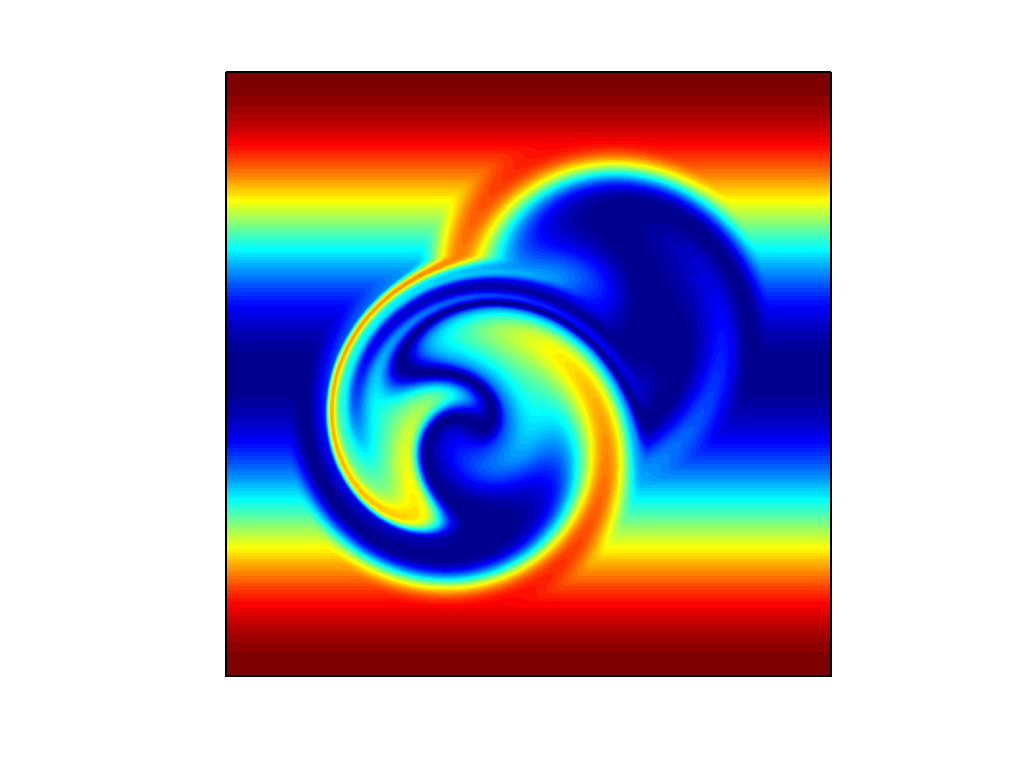
\includegraphics{ltmiter20.eps}}
  \scalebox{0.5}[0.5]{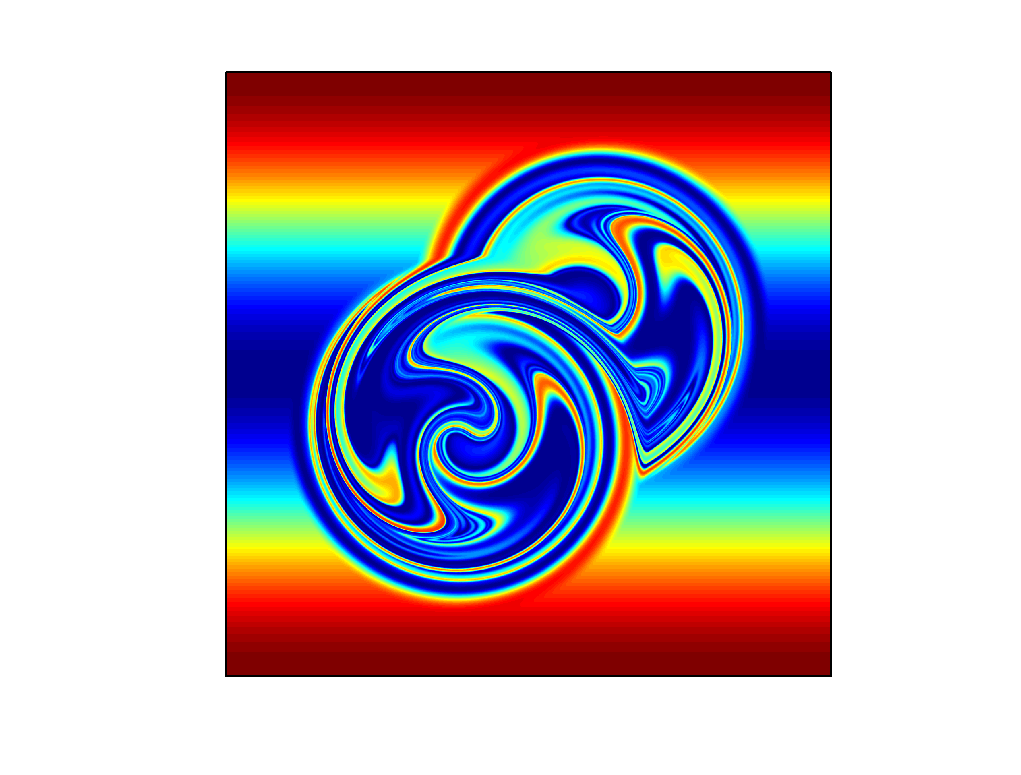
\includegraphics{ltmiter60.eps}}
  }
  \centerline{
  \scalebox{0.5}[0.5]{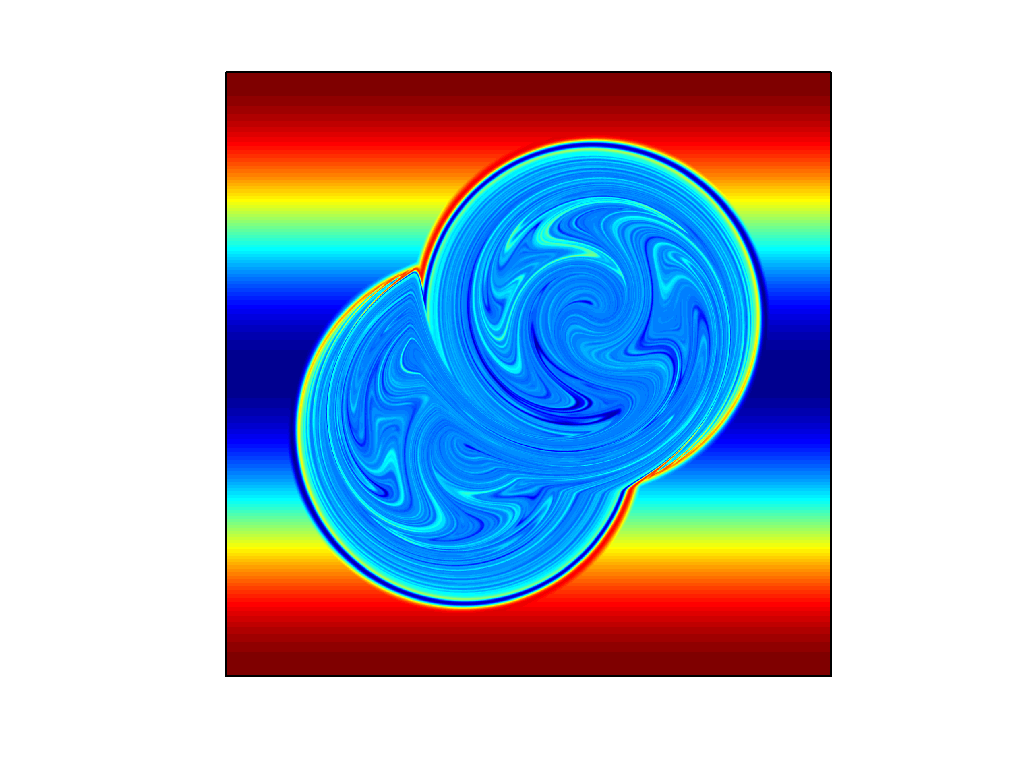
\includegraphics{ltmiter250.eps}}
  \scalebox{0.5}[0.5]{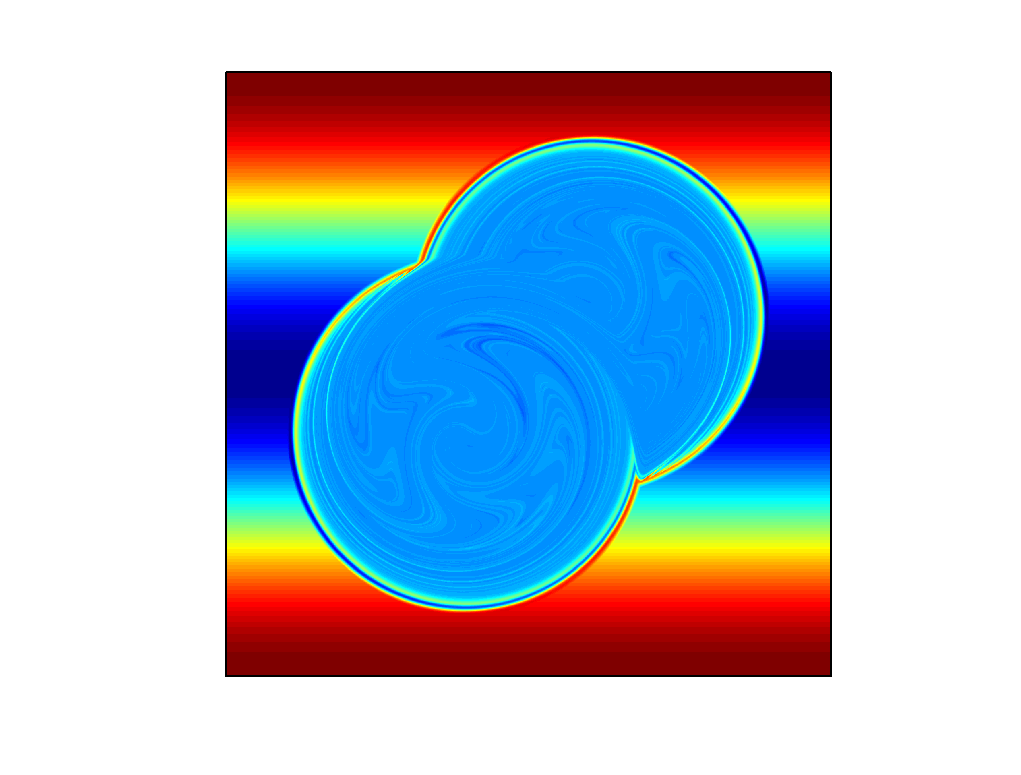
\includegraphics{ltmiter500.eps}}
  }
  \caption{LTM simulations with initial condition $c(x,y)=\cos(y)$,
          (a)iter=20, (b)iter=40, (c)iter=250, (d)=iter=500}
  \label{ltmiter}
\end{figure}


\begin{figure}
 \centerline{
  \scalebox{0.5}[0.5]{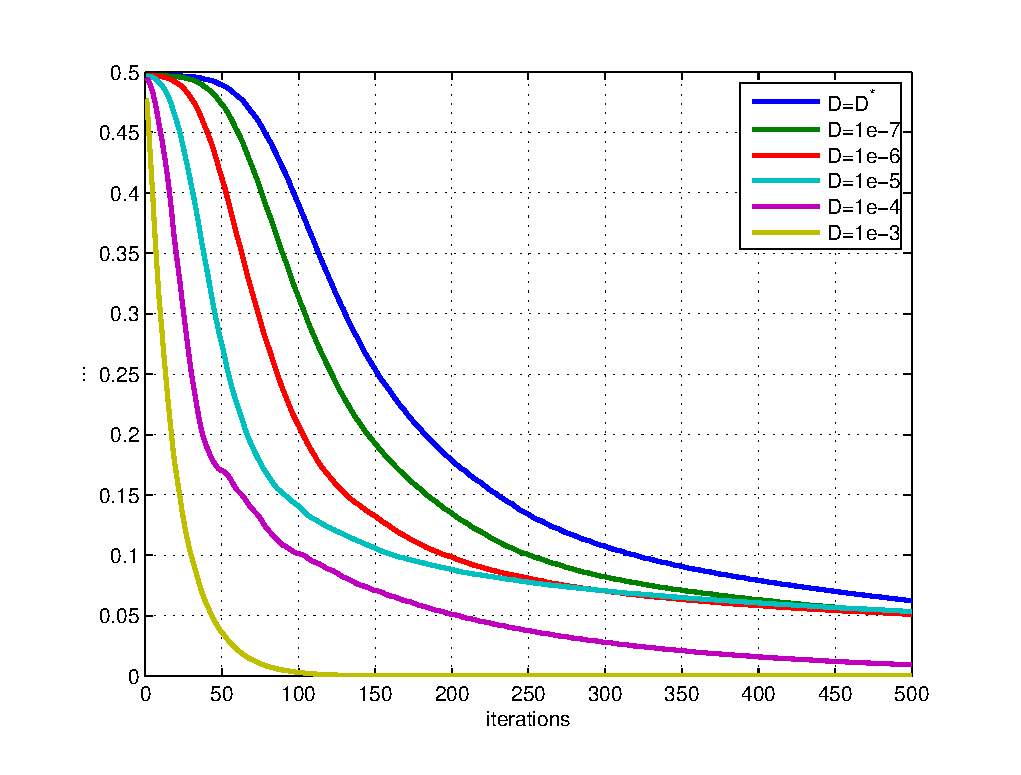
\includegraphics{ltmcutoff.eps}}
  } \caption{LTM}
  \label{LTM}
\end{figure}


\end{example}




%%%%%%%%%%%%%%%%%%%%%%%%%%%%%
\section{Remaining Questions}
%%%%%%%%%%%%%%%%%%%%%%%%%%%%%
%%%%%%%%%%%%%%%%%%%%%
\section{Conclusions}
\label{Conclusions}
%%%%%%%%%%%%%%%%%%%%%
We present a set of numerical simulations to show the cutoff behavior of standard map with decreasing diffusivity rates.
  


\cite{Wiggins2004}
\cite{Ottino2004}
\cite{Mezic2005}
\cite{Thiffeault2003-13}
\cite{Thiffeault2003-309}
\cite{Thiffeault2004}
\cite{Thiffeault2005}
\cite{Ashwin2002}
\cite{Boyd2004}
\cite{Diaconis1996}
\cite{Diaconis2001}
\cite{Diaconis2005}
\cite{Diaconis1986}
\cite{Hammarstr2005}
\cite{Fereday2002}
\cite{Tsang2005}
\cite{Haynes2005}
\cite{Pierrehumbert2000}
\cite{Percival1989}



% References
\bibliographystyle{plain}
\bibliography{mixingbib}

\end{document}
